%\documentclass[journal,12pt,draftclsnofoot,onecolumn]{IEEEtran} %draftclsnofoot
%\documentclass[confl, draftclsnofoot]{IEEEtran}
%\documentclass[conference,onecolumn,draft]{IEEEtran}
\documentclass[conference, 12pt]{IEEEtran}
\usepackage{fancyhdr}
\usepackage{grffile}
\usepackage{color}
\usepackage{graphicx}
\usepackage{cite}
\usepackage{multicol}
% \usepackage{subcaption}
\usepackage{algorithm}
\usepackage{algpseudocode}
\usepackage{pifont}
\usepackage{siunitx}
\usepackage{flushend}
\usepackage{amsmath}
\usepackage[hyphens]{url}
\usepackage{hyperref}

%\usepackage{setspace}
%\doublespacing
%\onecolumn
\begin{document}
%
% paper title
% can use linebreaks \\ within to get better formatting as desired
    \title{
        Minimal Viable Waterworld Agents:\\
        Experimenting with MultiAgent Reinforcement Learning
    }
%
%
% author names and IEEE memberships
% note positions of commas and nonbreaking spaces ( ~ ) LaTeX will not break
% a structure at a ~ so this keeps an author's name from being broken across
% two lines.
% use \thanks{} to gain access to the first footnote area
% a separate \thanks must be used for each paragraph as LaTeX2e's \thanks
% was not built to handle multiple paragraphs
%

    \author{Michael Hegerhorst}

% note the % following the last \IEEEmembership and also \thanks -
% these prevent an unwanted space from occurring between the last author name
% and the end of the author line. i.e., if you had this:
%
% \author{....lastname \thanks{...} \thanks{...} }
%                     ^------------^------------^----Do not want these spaces!
%
% a space would be appended to the last name and could cause every name on that
% line to be shifted left slightly. This is one of those "LaTeX things". For
% instance, "\textbf{A} \textbf{B}" will typeset as "A B" not "AB". To get
% "AB" then you have to do: "\textbf{A}\textbf{B}"
% \thanks is no different in this regard, so shield the last } of each \thanks
% that ends a line with a % and do not let a space in before the next \thanks.
% Spaces after \IEEEmembership other than the last one are OK (and needed) as
% you are supposed to have spaces between the names. For what it is worth,
% this is a minor point as most people would not even notice if the said evil
% space somehow managed to creep in.


% The paper headers
%\markboth{Journal of \LaTeX\ Class Files,~Vol.~6, No.~1, January~2007}%
%{Shell \MakeLowercase{\textit{et al.}}: Bare Demo of IEEEtran.cls for Journals}
% The only time the second header will appear is for the odd numbered pages
% after the title page when using the twoside option.
%
% *** Note that you probably will NOT want to include the author's ***
% *** name in the headers of peer review papers.                   ***
% You can use \ifCLASSOPTIONpeerreview for conditional compilation here if
% you desire.


% If you want to put a publisher's ID mark on the page you can do it like
% this:
%\IEEEpubid{0000--0000/00\$00.00~\copyright~2007 IEEE}
% Remember, if you use this you must call \IEEEpubidadjcol in the second
% column for its text to clear the IEEEpubid mark.


% use for special paper notices
%\IEEEspecialpapernotice{(Invited Paper)}


% make the title area
    \maketitle
%copyright notice
% TODO
% \thispagestyle{plain}
% \fancypagestyle{plain}{
%   \fancyhf{} % clear all header and footer fields
%   \fancyfoot[L]{978-1-4673-8988-4/17/\$31.00~\copyright2017~IEEE} % change
%       copyright notice here if required
%   \renewcommand{\headrulewidth}{0pt}
%   \renewcommand{\footrulewidth}{0pt}
% }

    \begin{abstract}
        Efficient metabolism in bioengineered tissues requires a robust vascular system to provide healthy microenvironments to the cells and stroma. Such networks form spontaneously during embryogenesis from randomly distributed endothelial cells. There is a need to bioengineer endothelial cells so that network formation and operation is optimal for synthetic tissues. This work introduces a computational model that simulates \textit{de novo} vascular development and assesses the effectiveness of the network in delivering nutrients and extracting waste from tissue. A genetic algorithm was employed to identify parameter values of the vaculogenesis model that lead to the most efficient and robust vascular structures. These parameter values control the behavior of cell-level mechanisms such as chemotaxis and adhesion. These studies demonstrate that genetic algorithms are effective at identifying model parameters that lead to near-optimal networks. This work suggests that computational modeling and optimization approaches may improve the effectiveness of engineered tissues by suggesting target cellular mechanisms for modification. 

    \end{abstract}


% IEEEtran.cls defaults to using nonbold math in the Abstract.
% This preserves the distinction between vectors and scalars. However,
% if the journal you are submitting to favors bold math in the abstract,
% then you can use LaTeX's standard command \boldmath at the very start
% of the abstract to achieve this. Many IEEE journals frown on math
% in the abstract anyway.

% Note that keywords are not normally used for peerreview papers.
    \renewcommand\IEEEkeywordsname{Key Words}
    \begin{IEEEkeywords}
% TODO
% Synthetic biology, self organization, vascular development, tissue engineering,
%         genetic algorithms, optimization, bioengineering.
    \end{IEEEkeywords}

% For peer review papers, you can put extra information on the cover
% page as needed:
% \ifCLASSOPTIONpeerreview
% \begin{center} \bfseries EDICS Category: 3-BBND \end{center}
% \fi
%
% For peerreview papers, this IEEEtran command inserts a page break and
% creates the second title. It will be ignored for other modes.
%\IEEEpeerreviewmaketitle

    \section{Introduction}\label{sec:introduction}
% What and why
% Problem statement
% Given: find: such that: (solving a problem)
% Question if a methodological study
Reinforcement learning is an extremely powerful tool that is able to solve a multitude
of problems.
One such toy problem is known as Waterworld~\cite{Karpathy2015, Ho2016}, which consists
of an agent chasing food and avoiding poison.
This problem has been expanded by~\cite{Gupta2017} to include multiple agents,
turning it into a multi-agent reinforcement learning problem with both cooperative
and competitive elements.
These agents receive readings from sensors connected to their bodies that
inform the agent on the distance of food, poison, obstacles, or other agents a sensor
is touching.
With some settings, these sensors also sense the speed of what they are touching.
The agent is also made aware when it eats food or poison.
The goal of Waterworld is to take the input of these sensors and find a way to apply
thrust to itself such that it consumes as much food as possible while avoiding poison
and with as little effort as possible.

Waterworld is a fascinating and complex problem with many ways to approach it.
An agent must learn how to move adeptly in a strange and ever-changing environment.
Wrong moves or a poorly planned trajectory will lead to the agent consuming poison
and receiving a significant negative reward.
Additionally, the agent is bombarded with a slew of information from the environment.
In the modern version provided by the Farama Foundation~\cite{WaterworldDocumentation},
agents receive $8 * \text{number of sensors} + 2$ or
$5 * \text{number of sensors} + 2$ (depending on settings) total observations.
With the default number of sensors being 30, this is a total of 242 (or 152)
observations!

While amount of input sounds like quite a bit, in the world of machine learning it is
not too much.
A small 32 x 32 image grayscale image would have 1024 observations, which is already
considerably larger.
Nevertheless, more observations means more processing time, and, when reinforcement
learning is used for robotics or other real world scenarios, additional sensors also
mean increased material or financial cost.
Additionally, the Waterworld agent's information is imperfect, and its observations
may appear to fluctuate almost randomly as food and poison brush against the sensors,
which increases the complexity.
As such, given a reinforcement learning problem, there is a need to determine how to
build an agent that is simple enough to minimize costs while still being complex.
enough to solve the problem.
In other words, one needs to find the ``sweet spot'' or ``Goldilocks zone'' in
complexity for the agent they are building.

    \section{Methods and Models}\label{sec:methods}
% RL method applied
% Experimental methods, (independent variables, dependent variables, control variables)
Waterworld has already been tackled by a number of authors.
Jonathan~Ho~et~al.~\cite{Ho2016} applied imitation learning (specifically, TRPO) to the
single-agent version of Waterworld using a unique model-free technique, and discovered
their technique showed promise.

Similarly, Jayesh~K.~Gupta~et~al.~\cite{Gupta2017} similarly applied a number of
reinforcement learning and imitation learning algorithms to the multi-agent version
of Waterworld and similar problems.
These algorithms include TRPO, A3C, and DDPG\@.
Each was applied using shared parameters, concurrent, and centralized techniques.
They discovered parameter-sharing A3C yielded the best results for Waterworld, while
TRPO performed best for centralized.
A3C was the only successful model for concurrent.

\subsection{Training Algorithms and Agent Types}\label{subsec:training-algorithms}
In this study, we apply three common reinforcement learning algorithms, as well as a
basic controls-agent hybrid, to train our agents.
All algorithms use a deep neural network at some point of their operation.
Specifically, we use a continuous-space adapted Q-learning algorithm, as well as A2C,
and DDPG in addition to the hybrid.
We are not using TPRO because, as outlined by~\cite{Ho2016}, imitation learning tends
to have difficulty with complex environments and higher-dimensional states.
While the same authors outlined ways to overcome this obstacle, imitation learning
also relies on having some ``expert'' to show the agent how to act.
These experts are not always available, and so, in order to generalize our findings,
we will avoid using imitation learning except for the controls-agent hybrid.

\subsubsection{Q-learning (QNN)}
The Q-learning algorithm works as a stacked Q-learning neural network (or QNN).
Each action dimension has its own policy QNN, which receive the same input.
Each policy has $n_\pi$ outputs, where $n >= 2$.
Since Q-learning works with probabilities for discrete actions, the continuous
action space over which the policy operates is divided into $n_\pi$ equal partitions,
with each output being associated with one partition.
For example, if the continuous actions space interval were $[-1, 1]$ (as it is for
Waterworld), and a policy has 5 outputs, the partitions would be $-1.0, -0.5, 0.0, 0.5,
\text{ and } 1.0$.
The partition with the highest associated output is selected as the action for that
dimension.
Essentially, the continuous space is converted to a discrete space that works with
the QNN\@.

\subsubsection{Advantage Actor-Critic (A2C)}
A2C, or Advantage Actor-Critic, works similarly to the Q-learning agent.
Each action dimension has an associated policy, and the policy outputs are used to
choose which partition of the discretized space to use.
The primary difference between the two is A2C uses a policy ``goodness'' or
``advantage'' network, called a \textit{critic}, to determine how good the current
and next states are.
The critic learns in parallel with the actor.
Additionally, both the policy and advantage networks can use a shared network to as
part of their computations.

This setup allows for the agent to determine its own advantage function, which
allows the system to more easily learn complex problems.

\subsubsection{Deep Deterministic Policy Gradient (DDPG)}
DDPG operates by having a policy model, called an \textit{actor}, and a ``goodness''
model, again called a \textit{critic}.
The actor is able to output continuous values, allowing for more fine-tuned control
than the discrete-space algorithms.
As with A2C, the critic determines the ``goodness'' of states, except in DDPG the
critic determines the ``goodness'' of an action for a state, giving it more control
over how the agent operates.
The critic also trains in parallel with the actor.

\subsubsection{Controls-Agent Hybrid (CPT)}\label{subsubsec:cpt}
The controls-agent hybrid, or Controls Policy Trainer (CPT) is used to develop a critic
model for DDPG\@.
It simply thrusts towards food, and away from poison if it cannot find any food.
This ``agent'' serves as both to show how much reward is possible, as well as train a
critic for DDPG\@.
The hope is to be able to create a strong critic before the DDPG actor starts
training, thereby jumpstarting the process.
The critic developed can then continue training with DDPG, or be locked.
Locking the critic will have the side effect that the actor will always be attempting
to mimic the controller algorithm instead of determining an alternative, higher value
solution.

\subsection{Model Architecture}\label{subsec:model-architecture}
Each algorithm uses one or more neural networks.
Each neural network we use falls into one of three categories: standard, distance, or
critic.
The primary difference between these categories is how the handle the incoming state,
or observation.

\subsubsection{Standard Networks}
Standard networks are simple sequential networks.
They take input and pass it from layer to layer.
They can include more complex components, such as convolutional or LSTM layers, but
they ultimately work as sequential networks that take input and pass between layers
without any additional processing.
Most of the standard networks we use consist of only linear layers.

\subsubsection{Distance Networks}
Distance networks specifically extract the distance parameters from the environment
observations.
These distance observations are then piped into a separate network before rejoining the
rest of the observation.
The hope behind this style of network is to allow the agent to apply different
calculations on the distance parameters, in particular convolutions, in order to better
interpret them.

\subsubsection{Critic Networks}
Critic networks are special networks specifically built for the DDPG and
Controls-Agent Hybrid agents types.
They are meant to determine the ``goodness'' of an action for a given observation,
and so receive both the observation and action as input.
They can contain the other types of networks to take advantage of their features.

\subsection{Memory}\label{subsec:memory}
Memory is an important aspect of how the agent learns.
Without memory, the agent would only be able to learn from the current state, and
not learn how to get to that state.
However, rewards in Waterworld are somewhat sporadic and
sparse~(\autoref{fig:example-episode-rewards}), which makes it difficult for the
agent to learn which actions are good and which are bad.

\begin{figure}[htbp]
    \centering
    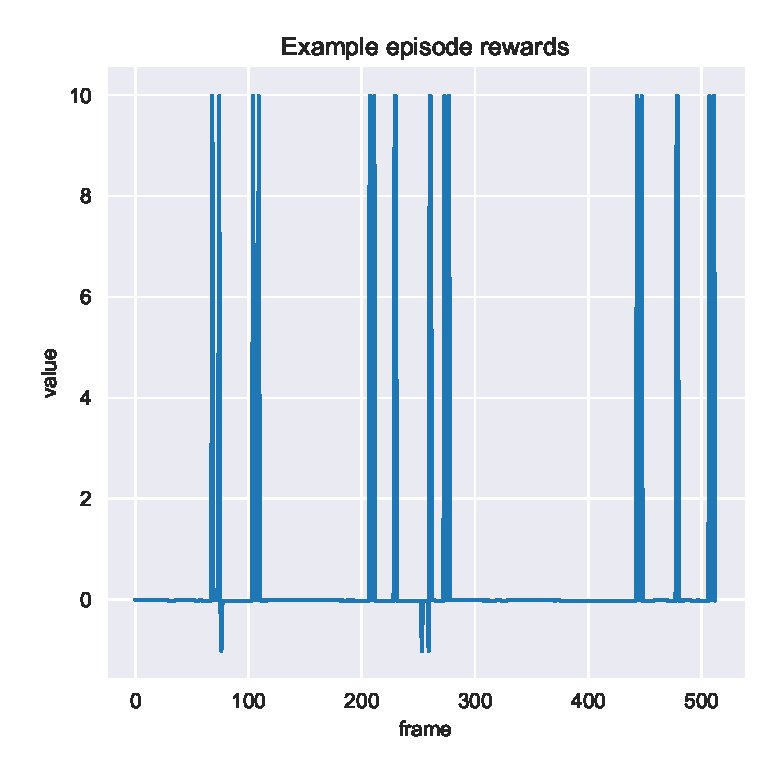
\includegraphics[scale=0.75]
    {./figures/example-episode-rewards}
    \caption{
        Example of instantaneous rewards for a single episode.
        The x-axis shows the frame, or step, when the reward was received, and the
        y-axis shows the reward.
        The high spikes are when the agent manages to eat food, while the low spikes
        are when the agent eats poison.
        Very slight dips can be seen as well, which are when the agent applies thrust.
    }
    \label{fig:example-episode-rewards}
\end{figure}

With this in mind, we developed two different types of memory: standard memory and
reward prioritized memory.

\subsubsection{Standard Memory}
Standard memory simply keeps track of the current state, actions, rewards, and next
states.
It can be sampled to return one or more record, which can then be used to train the
agent.

\subsubsection{Reward Prioritized Memory}
Reward prioritized memory is a special type of memory that, as with standard memory,
keeps track of the current state, actions, rewards, and next states.
However, it uses a simple algorithm to determine which records are more important/rare
than others and is more likely to return those memories when sampled.

The algorithm used to determine the rarity of a memory is simple.
A mean reward of 0 and a standard deviation of 0 are initialized.
Whenever a record is added to the memory buffer, the mean reward is updated as well as
the standard deviation.
When the memory is sampled, the z-score for each record is calculated and serves as
the record's weight.
Once all z-scores are calculated, the weights are used to randomly select samples
from the buffer.

The hope behind this structure was to emphasize those rare rewards and punishments in
an effort to accelerate learning and guide the agent towards the observations that
will most benefit the agent.

\subsection{Analysis Methods}\label{subsec:analysis-methods}
Analyses for this study were primarily based on total episode reward and the time it
took for an agent to settle.
Graphs were generated throughout training to monitor an agent's progress.
Whereas Waterworld each run is starts with random variables, some smoothing will then
be applied to these graphs to focus on general trends.

We will focus on four different analyses: Agent Type, Memory Type, Architecture, and
CPT\@.
The Agent Type portion will focus on the performance of different agents, as 
described in \autoref{subsec:training-algorithms}.
Likewise, Memory Type will focus on Reward Prioritized Memory vs Normal Memory, as 
described in \autoref{subsec:memory}, and Architecture will focus on Standard Networks
vs Distance Networks.
Whereas Waterworld has a time component, the Architecture section will also 
experiment with these networks with LSTM layers.
Finally, CPT will compare a DDPG Distance actor against a DDPG Distance actor trained
using a policy generated by \hyperref[subsubsec:cpt]{CPT}.

Agents with each combination of agent type, memory type, and architecture will be run
for the same number of iterations.
Afterwords, groupings will be made according to the analysis, and averages of rewards
and losses calculated.
Afterwards, graphs will be made to determine what difference, if any, there is for
each group.

% TODO: come back to this after finishing the results section.

    \section{Results}\label{sec:results}

\subsection{Agent Type}\label{subsec:agent-type}
The average rewards by agent type can be seen in \autoref{fig:rewards-by-agent}.
Unfortunately, none of the agents were able to do as well as the controller used by the
CPT\@.
Additionally, all agents performed as bad or worse as a simple random controller!
It is possible that this problem is complex enough that the models needed more time
to train, but no significant additional gains were made when training for over 12,000
episodes, so there appears to be something wrong.

\begin{figure}[!ht]
    \centering
    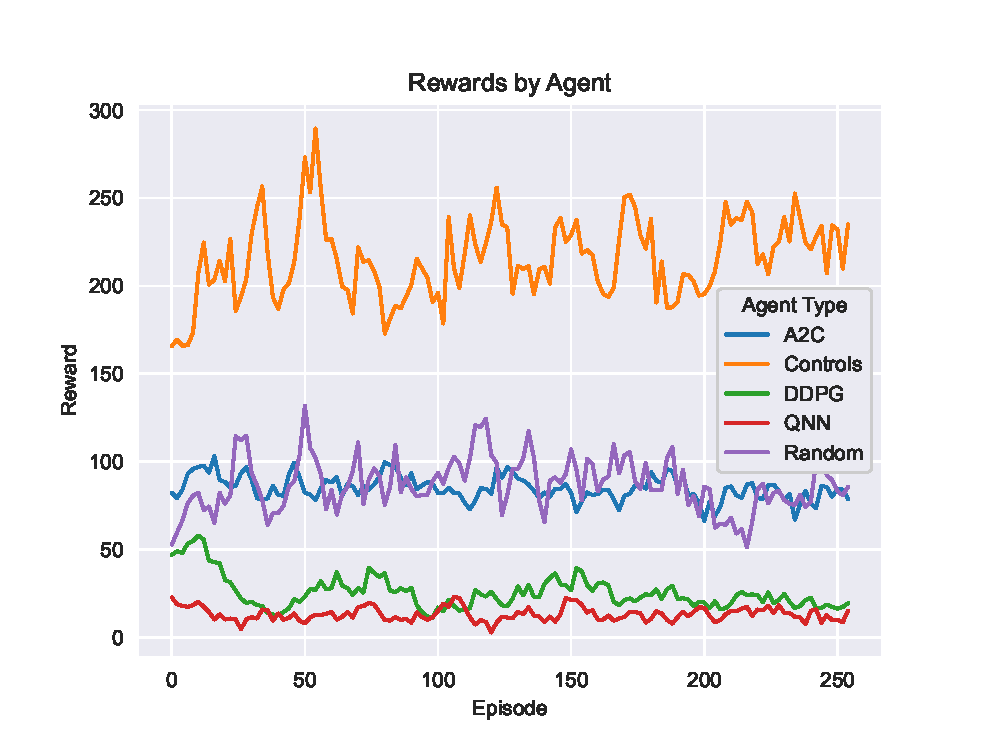
\includegraphics[scale=0.5]
    {./figures/rewards-by-agent}
    \caption{
        Rewards by agent type.
        The x-axis is the episode, while the y-axis is the reward.
    }
    \label{fig:rewards-by-agent}
\end{figure}

Interestingly, the A2C agents seems to perform the best out of all the agents used.
DDPG seems to perform second best, while QNN performs the worst.
Further work should be done to determine why these agents aren't improving and what
changes need to be made to improve them.
The average reward for each agent is shown in \autoref{tab:agent-average-reward}.

\begin{table}[!htbp]
    % increase table row spacing, adjust to taste
    \renewcommand{\arraystretch}{1.3}

    \caption{The average rewards by agent type.}
    \label{tab:agent-average-reward}

    \centering
    \begin{tabular}{|c|c|}
        \hline
        Agent    & Average Reward \\
        \hhline{|=|=|}
        A2C      & 84.77          \\
        \hline
        Controls & 216.75         \\
        \hline
        DDPG     & 25.05          \\
        \hline
        QNN      & 13.04          \\
        \hline
        Random   & 87.68          \\
        \hline
    \end{tabular}
\end{table}

\subsection{Memory Type}\label{subsec:memory-type}
The loss by memory type is displayed per agent type in \autoref{fig:loss-by-memory}.
Specifically, the loss for the actor is used in the case of A2C and DDPG, while QNN
simply displays ``loss'' since it itself is the actor.

\begin{figure}[!ht]
    \centering
    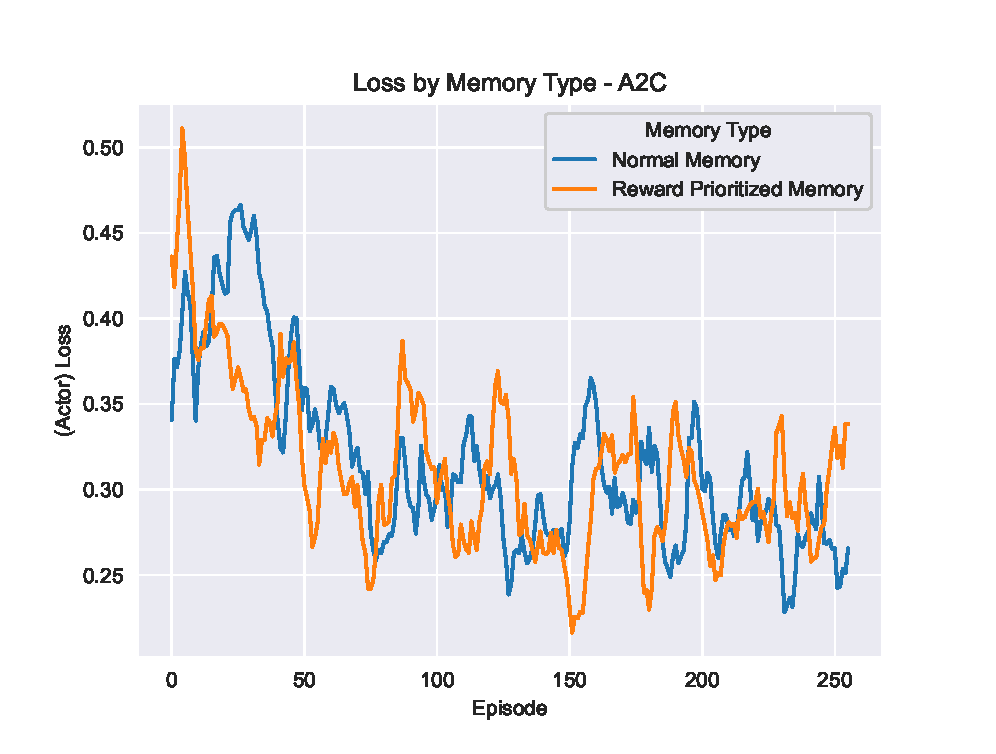
\includegraphics[scale=0.5]
    {./figures/memory/loss-by-memory-A2C}
    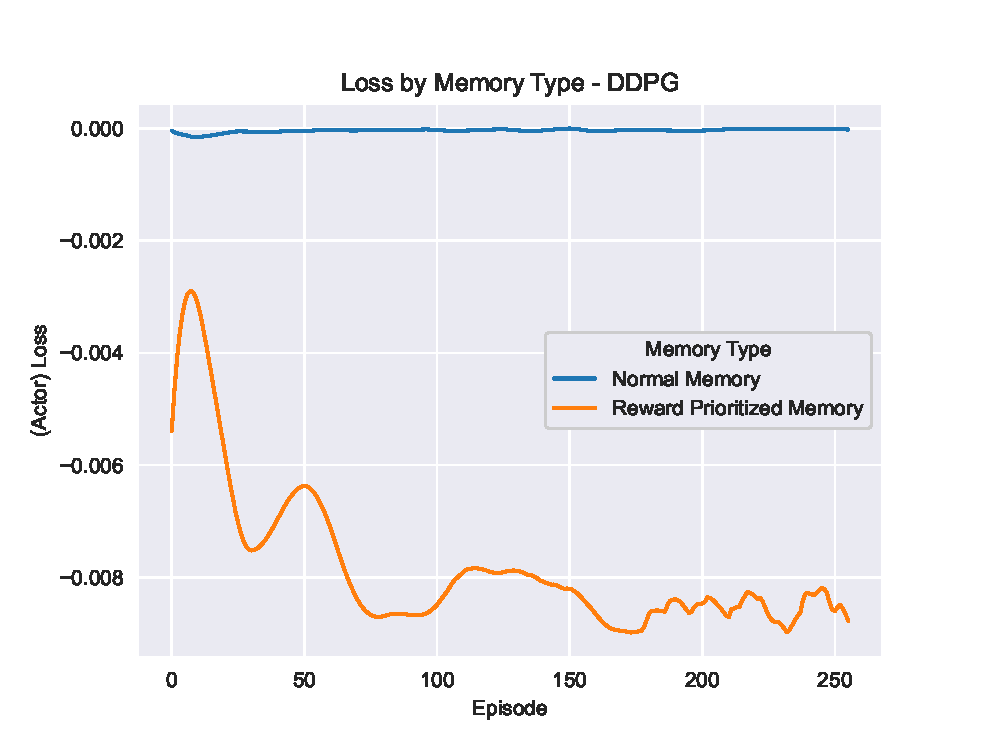
\includegraphics[scale=0.5]
    {./figures/memory/loss-by-memory-DDPG}
    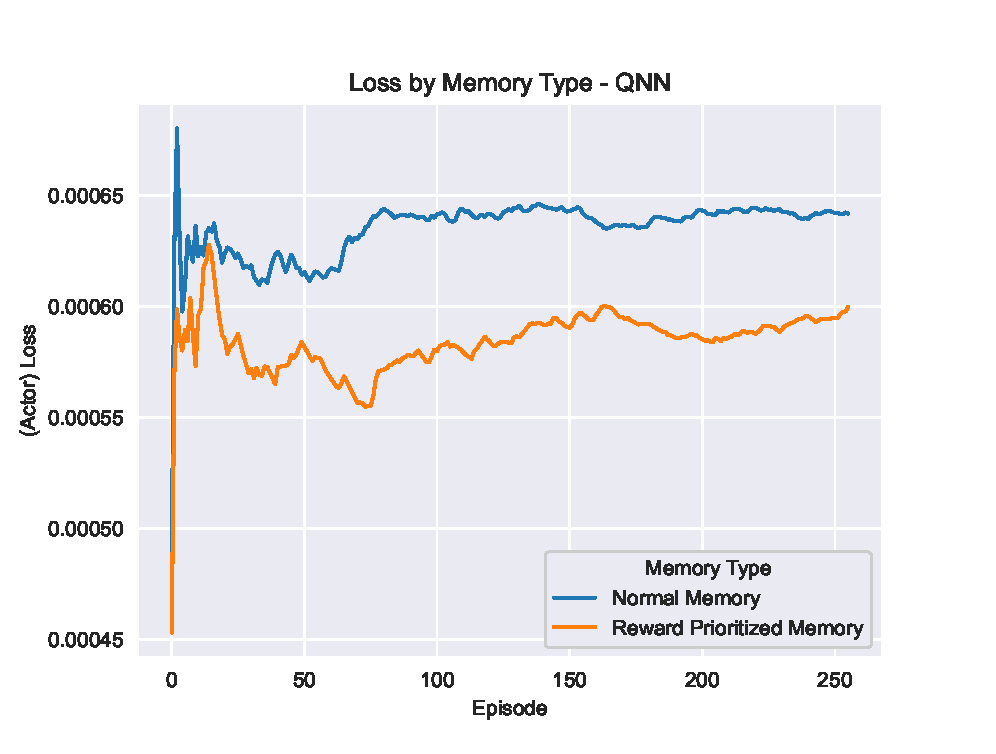
\includegraphics[scale=0.5]
    {./figures/memory/loss-by-memory-QNN}
    \caption{
        Loss by memory type for each agent type.
        The x-axis is the episode, while the y-axis is the loss.
        Lower loss is better than higher loss.
    }
    \label{fig:loss-by-memory}
\end{figure}

RPM initially appears to provide better gains in terms of loss.
Specifically, there is an initial dip in loss, but then the slopes of RPM and normal
memory seem to converge.
DDPG especially seems to gain a huge benefit from RPM, but it should be noticed that
for all agents the advantage provided by RPM is fairly small, typically only
consisting of hundredths of decimal places, if that.
Additional experiments should be performed to confirm the effectiveness, or lack
thereof, of Reward Prioritized Memory.

\subsection{Architecture}\label{subsec:architecture}

\subsection{DDPG with CPT}\label{subsec:ddpg-with-cpt}

    \section{Summary}\label{sec:summary}

    \section{Conclusions}\label{sec:conclusions}

    % TODO
    % Sources
    %   Citations to papers
    %   Links to websites
    %   Code sources
    %   How to publish, link to your own webpage, git hub page, etc.

    \bibliographystyle{IEEEtran}

    \begin{small}

        \bibliography{references}

    \end{small}


\end{document}
